\section{Versuchsaufbau}
%skizze zum versuchsaufbau (oder foto) einf�gen,   es muss erkl�rt werden wie das ganze funktioniert und welche speziellen einstellungen verwendet wurden (z.b. welche kn�pfe an den ger�ten f�r die messung verdreht wurden)
\label{sec:versuchsdurchf�hrung}
In diesem Abschnitt wird der Aufbau des Rastertunnelmikroskops beschrieben. Das Rastertunnelmikroskop basiert auf dem in Abschnitt ?? beschriebenem Tunneleffekt. Die leitende Spitze des Rastertunnelmikroskops wird hinreichend nah an die Oberfl�che des zu untersuchendes Material gef�hrt, ber�hrt diese jedoch nicht. Wird eine Spannung angelegt, so kann ein ``Tunnelstrom'' flie�en. Bewegt man nun die Spitze nun Parallel zur Oberfl�che, so erh�lt �ber den Tunnelstroms ortaufgel�ste Informationen �ber die Oberfl�che.

Grundlegend ist das Rastertunnelmikroskop aus drei Elementen aufgebaut, einem Tastkopf, einem Piezosteuerelement und einer Probe. Der Tastkopf besteht aus einem Draht, mit einer Spitze, die m�glichst einatomig sein soll. Durch die Dicke der Spitze wird das Aufl�sungsverm�gen des Mikroskops festgelegt. In diesem Versuch wird ein Platin-Iridium-Draht als Tastkopf verwendet. Das Piezosteuerelement dient zur Positionierung der Spitze. Dabei kann der Tastkopf im nm-Bereich verschoben werden. F�r die Untersuchung einer Oberfl�che mit einem Rastertunnelmikroskops muss die Probe bestimmte Eigenschaften erf�llen. Die Probe muss ein Leiter oder ein Halbleiter sein. Da beschichten der Oberfl�che mit einem leitendem Material ist nicht m�glich, da die Oberfl�chenstrucktur durch die Beschichtung die Oberfl�chen verdeckt wird. 

Ein schematischer Versuchsaufbau ist in Abbildung \ref{fig:aufbau} zu sehen.

\begin{figure}[H]
	\centering
  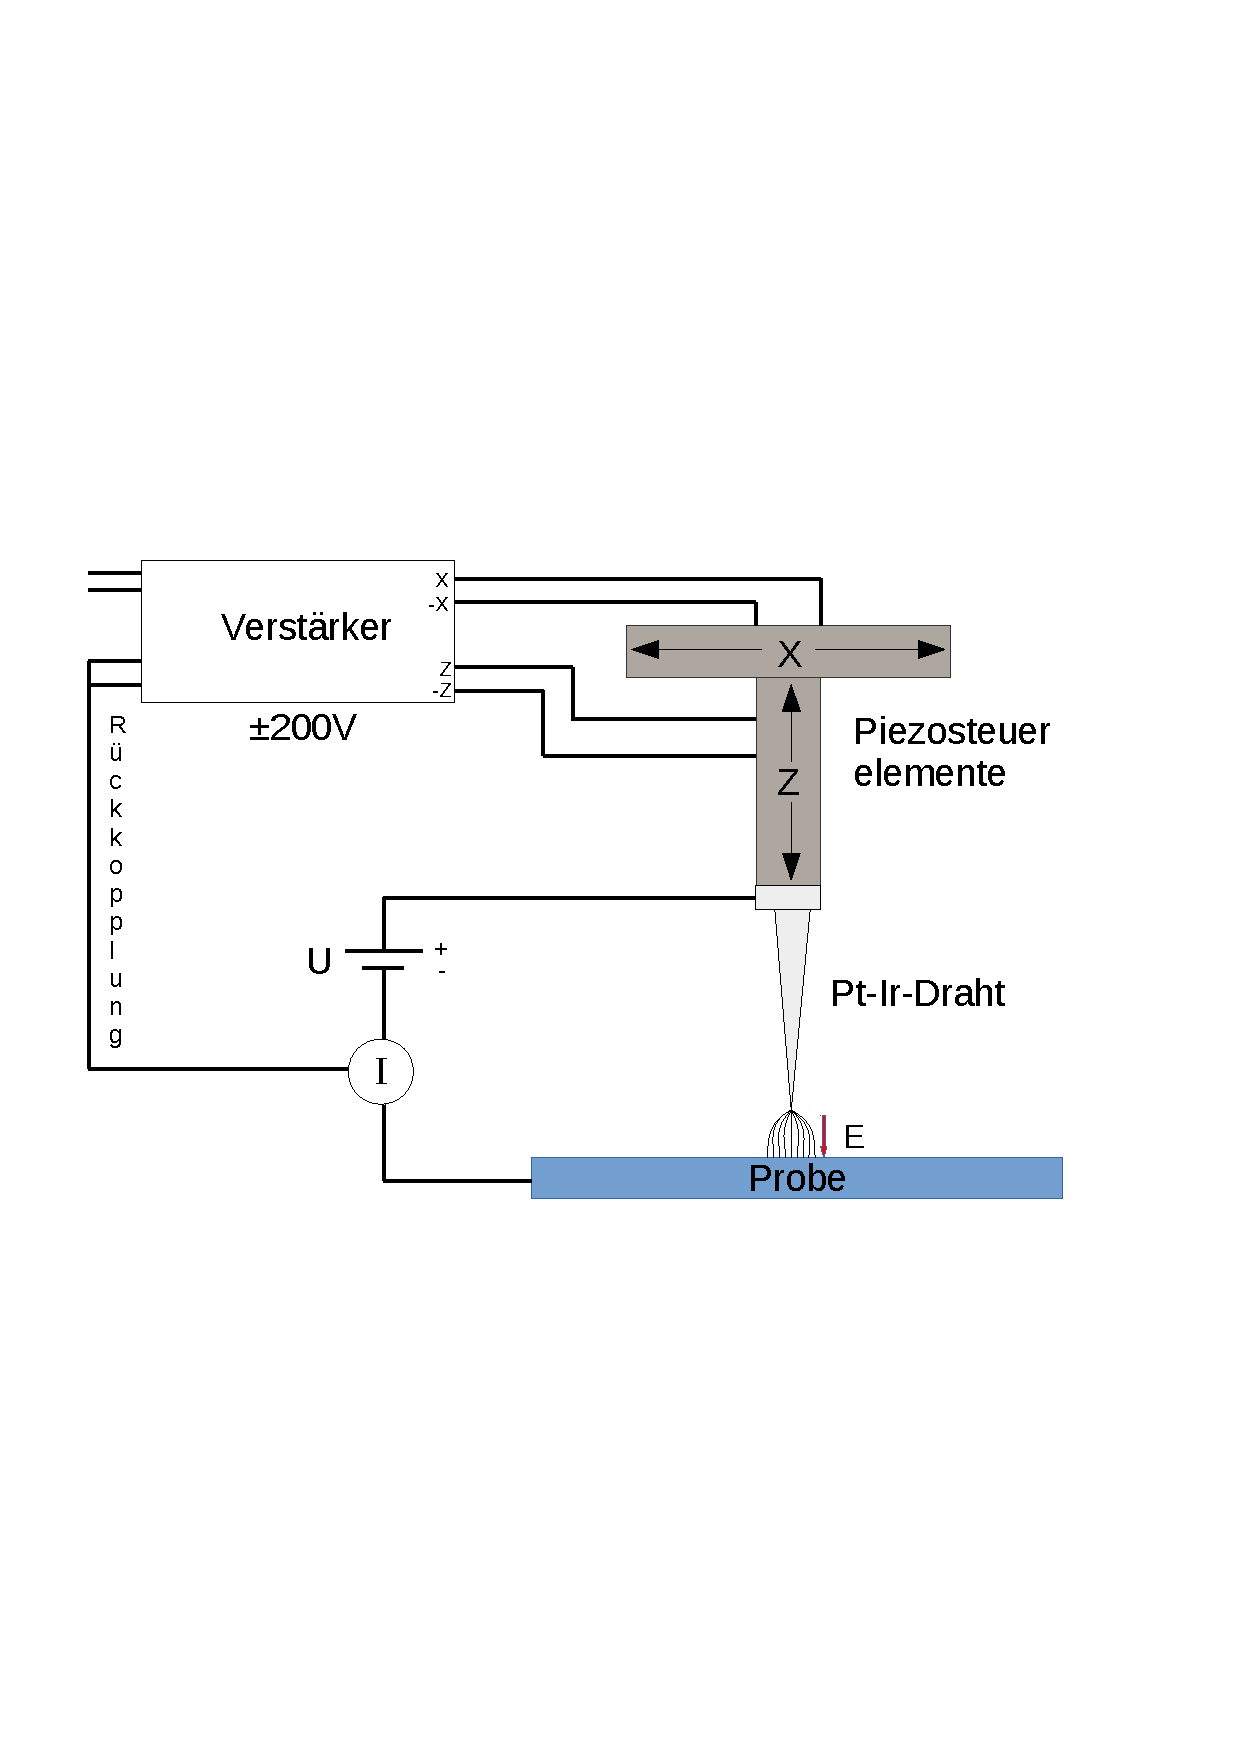
\includegraphics[trim = 10mm 90mm 30mm 90mm, clip, scale=0.8]{aufbau.pdf}
	\caption{Schematische Skizze des Versuchsaufbaus. Die Positionierung der Platin-Iridium-Tastkopes wird �ber die Piezoelemente im nm-Bereich gesteuert. Die R�ckkopplung dient zur Steuerung der H�he des Tastkopfes.}
	\label{fig:aufbau}
\end{figure}



